En la guía se utiliza el comando \textit{guide} para implementar una interfaz. El tema es que dicho comando quedó en deshuso ya que el sistema migró a \textit{App Designer}\footnote{\url{https://la.mathworks.com/products/matlab/app-designer.html}}. Esto conllevó a usar la inteligencia artificial ya que muchos de los comandos que implementa la guía no existen más. Se utilizó \textit{ChatGPT} para replicar lo mismo que la guía. Se detalla el paso a paso para implementar dicha interfaz o app:

\begin{enumerate}
    \item \textbf{Colocamos los elementos en la interfaz}: \textit{Static Text} se conoce como \textit{Label}; \textit{Edit Text} se conoce como \textit{Edit Field (Text)}; \textit{Pop-up Menu} se conoce como \textit{Drop Down}; \textit{Push Button} se conoce como \textit{Button} y el \textit{Axes} sigue igual.
    
    \begin{figure}[ht!]
        \centering
        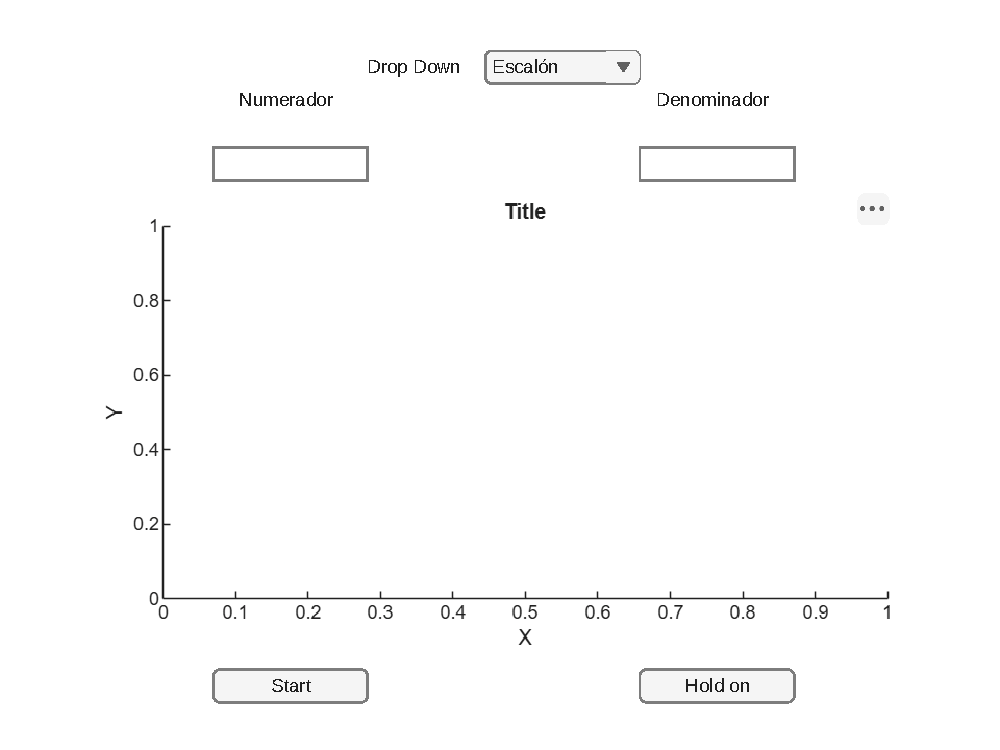
\includegraphics[width=0.8\textwidth]{imagenes/interfaz.pdf}
        \caption{Colocación de los elementos en mi interfaz gráfica}
        \label{fig:1}
    \end{figure}
    
    \item \textbf{Creación de las propiedades}: En Code View, abrimos Editor → Property → Private Property. App Designer crea un bloque properties (Access = private). Agregamos lo siguiente:
    
    \begin{lstlisting}
    properties (Access = private)
        N = []
        D = []
        v = 'Escalon'
    end
    \end{lstlisting}

    \texttt{N} es el numerador, \texttt{D} es el denominador y \texttt{v} es la entrada. 

    \item \textbf{Creamos los callbacks}: En Design View, buscamos app.numEditField en el panel derecho Component Browser. Hacemos clic derecho sobre ese componente y elegimos Callbacks → Add ValueChangedFcn callback. App Designer va a crear la función y nos lleverá a su parte editable. Hacemos lo mismo con el denominador y el desplegable (Dropdown):
    
    \begin{lstlisting}
    % Value changed function: numEditField
        function numEditFieldValueChanged(app, event)
            app.N = str2num(app.numEditField.Value, Evaluation="restricted");
            disp(app.N)
        end

        % Value changed function: denEditField
        function denEditFieldValueChanged(app, event)
            app.D = str2num(app.denEditField.Value, Evaluation="restricted");
            disp(app.D)
        end

        % Value changed function: DropDown
        function DropDownValueChanged(app, event)
            app.v = app.DropDown.Value;
            
        end
    \end{lstlisting}
    
    \item \textbf{Superponer las curvas}: Clic derecho sobre app.HoldonButton → Callbacks → Add ButtonPushedFcn callback. Pegamos este código dentro de la función generada. Hacemos lo mismo con el botón de Start:
    
    \begin{lstlisting}
     % Button pushed function: HoldonButton
        function HoldonButtonPushed(app, event)
            if ishold(app.UIAxes)
                hold(app.UIAxes, 'off');
                app.HoldonButton.Text = 'Hold on';
            else
                hold(app.UIAxes, 'on');
                app.HoldonButton.Text = 'Hold off';
            end
        end

        % Button pushed function: StartButton
        function StartButtonPushed(app, event)
            try
                N = app.N;
                D = app.D;

                if isempty(N) || isempty(D)
                    error('Ingresa coeficientes numericos en ambos campos. Ejemplo: 1 2 1');
                end

                validateattributes(N, {'numeric'}, {'row', 'real', 'finite'}, '', 'Numerador');
                validateattributes(D, {'numeric'}, {'row', 'real', 'finite'}, '', 'Denominador');

                if all(D == 0)
                    error('El denominador debe tener al menos un coeficiente distinto de cero.');
                end

                sis = tf(N, D);

                switch app.v
                    case 'Escalon'
                        [y, t] = step(sis);
                    case 'Impulso'
                        [y, t] = impulse(sis);
                    otherwise
                        uialert(app.UIFigure, 'Elegi Escalon o Impulso.', 'Tipo de entrada');
                        return
                end

                plot(app.UIAxes, t, y, 'LineWidth', 1.5);
                grid(app.UIAxes, 'on');
                xlabel(app.UIAxes, 'Tiempo (s)');
                ylabel(app.UIAxes, 'Salida');
                title(app.UIAxes, 'Respuesta del sistema');

            catch ME
                uialert(app.UIFigure, ME.message, 'Error al calcular la respuesta');
            end
        end
    \end{lstlisting}
    \item \textbf{Prueba}: Ingresemos la siguiente función de transferencia y probamos con una entrada escalón e impulso:
    
    \begin{equation}
        G(s) = \frac{1}{s^2 + s + 1}
    \end{equation}

    \begin{figure}[ht!]
        \centering
        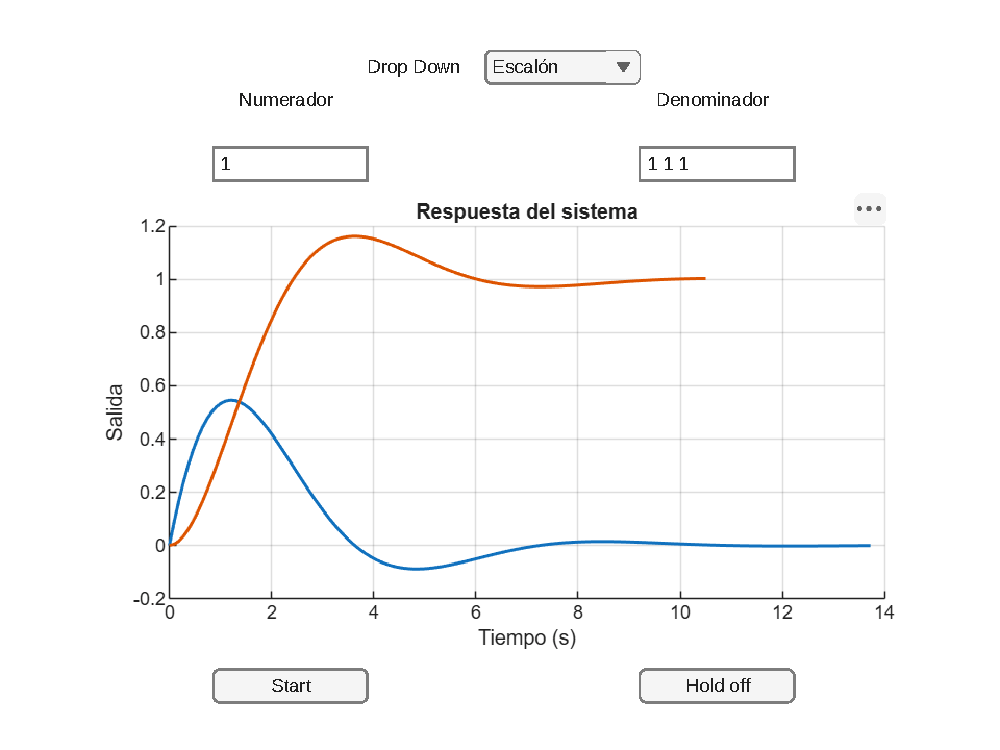
\includegraphics[width=0.9\textwidth]{imagenes/prueba.pdf}
        \caption{La curva azul representa a la respuesta impulso y la naranja al escalón}
        \label{fig:2}
    \end{figure}
    
\end{enumerate}

\newpage

El código completo es:

\begin{lstlisting}
classdef app1 < matlab.apps.AppBase

    % Properties that correspond to app components
    properties (Access = public)
        UIFigure          matlab.ui.Figure
        StartButton       matlab.ui.control.Button
        HoldonButton      matlab.ui.control.Button
        DropDown          matlab.ui.control.DropDown
        DropDownLabel     matlab.ui.control.Label
        DenominadorLabel  matlab.ui.control.Label
        numerador         matlab.ui.control.Label
        denEditField      matlab.ui.control.EditField
        numEditField      matlab.ui.control.EditField
        UIAxes            matlab.ui.control.UIAxes
    end

    
    properties (Access = private)
        N = []
        D = []
        v = 'Escalon'
    end
    

    % Callbacks that handle component events
    methods (Access = private)

        % Value changed function: numEditField
        function numEditFieldValueChanged(app, event)
            app.N = str2num(app.numEditField.Value, Evaluation="restricted");
            disp(app.N)
        end

        % Value changed function: denEditField
        function denEditFieldValueChanged(app, event)
            app.D = str2num(app.denEditField.Value, Evaluation="restricted");
            disp(app.D)
        end

        % Value changed function: DropDown
        function DropDownValueChanged(app, event)
            app.v = app.DropDown.Value;
            
        end

        % Button pushed function: HoldonButton
        function HoldonButtonPushed(app, event)
            if ishold(app.UIAxes)
                hold(app.UIAxes, 'off');
                app.HoldonButton.Text = 'Hold on';
            else
                hold(app.UIAxes, 'on');
                app.HoldonButton.Text = 'Hold off';
            end
        end

        % Button pushed function: StartButton
        function StartButtonPushed(app, event)
            try
                N = app.N;
                D = app.D;

                if isempty(N) || isempty(D)
                    error('Ingresa coeficientes numericos en ambos campos. Ejemplo: 1 2 1');
                end

                validateattributes(N, {'numeric'}, {'row', 'real', 'finite'}, '', 'Numerador');
                validateattributes(D, {'numeric'}, {'row', 'real', 'finite'}, '', 'Denominador');

                if all(D == 0)
                    error('El denominador debe tener al menos un coeficiente distinto de cero.');
                end

                sis = tf(N, D);

                switch app.v
                    case 'Escalon'
                        [y, t] = step(sis);
                    case 'Impulso'
                        [y, t] = impulse(sis);
                    otherwise
                        uialert(app.UIFigure, 'Elegi Escalon o Impulso.', 'Tipo de entrada');
                        return
                end

                plot(app.UIAxes, t, y, 'LineWidth', 1.5);
                grid(app.UIAxes, 'on');
                xlabel(app.UIAxes, 'Tiempo (s)');
                ylabel(app.UIAxes, 'Salida');
                title(app.UIAxes, 'Respuesta del sistema');

            catch ME
                uialert(app.UIFigure, ME.message, 'Error al calcular la respuesta');
            end
        end
    end

    % Component initialization
    methods (Access = private)

        % Create UIFigure and components
        function createComponents(app)

            % Create UIFigure and hide until all components are created
            app.UIFigure = uifigure('Visible', 'off');
            app.UIFigure.Color = [1 1 1];
            app.UIFigure.Position = [100 100 640 480];
            app.UIFigure.Name = 'MATLAB App';
            app.UIFigure.Theme = 'light';
            app.UIFigure.WindowStyle = 'alwaysontop';
            app.UIFigure.WindowState = 'minimized';

            % Create UIAxes
            app.UIAxes = uiaxes(app.UIFigure);
            title(app.UIAxes, 'Title')
            xlabel(app.UIAxes, 'X')
            ylabel(app.UIAxes, 'Y')
            zlabel(app.UIAxes, 'Z')
            app.UIAxes.Position = [68 66 506 290];

            % Create numEditField
            app.numEditField = uieditfield(app.UIFigure, 'text');
            app.numEditField.ValueChangedFcn = createCallbackFcn(app, @numEditFieldValueChanged, true);
            app.numEditField.Position = [137 365 100 22];

            % Create denEditField
            app.denEditField = uieditfield(app.UIFigure, 'text');
            app.denEditField.ValueChangedFcn = createCallbackFcn(app, @denEditFieldValueChanged, true);
            app.denEditField.Position = [410 365 100 22];

            % Create numerador
            app.numerador = uilabel(app.UIFigure);
            app.numerador.Position = [154 406 65 22];
            app.numerador.Text = 'Numerador';

            % Create DenominadorLabel
            app.DenominadorLabel = uilabel(app.UIFigure);
            app.DenominadorLabel.Position = [421 406 77 22];
            app.DenominadorLabel.Text = 'Denominador';

            % Create DropDownLabel
            app.DropDownLabel = uilabel(app.UIFigure);
            app.DropDownLabel.HorizontalAlignment = 'right';
            app.DropDownLabel.Position = [231 427 65 22];
            app.DropDownLabel.Text = 'Drop Down';

            % Create DropDown
            app.DropDown = uidropdown(app.UIFigure);
            app.DropDown.Items = {'Entrada', 'Escalon', 'Impulso'};
            app.DropDown.ValueChangedFcn = createCallbackFcn(app, @DropDownValueChanged, true);
            app.DropDown.Position = [311 427 100 22];
            app.DropDown.Value = 'Escalon';

            % Create HoldonButton
            app.HoldonButton = uibutton(app.UIFigure, 'push');
            app.HoldonButton.ButtonPushedFcn = createCallbackFcn(app, @HoldonButtonPushed, true);
            app.HoldonButton.Position = [410 31 100 22];
            app.HoldonButton.Text = 'Hold on';

            % Create StartButton
            app.StartButton = uibutton(app.UIFigure, 'push');
            app.StartButton.ButtonPushedFcn = createCallbackFcn(app, @StartButtonPushed, true);
            app.StartButton.Position = [137 31 100 22];
            app.StartButton.Text = 'Start';

            % Show the figure after all components are created
            app.UIFigure.Visible = 'on';
        end
    end

    % App creation and deletion
    methods (Access = public)

        % Construct app
        function app = app1

            % Create UIFigure and components
            createComponents(app)

            % Register the app with App Designer
            registerApp(app, app.UIFigure)

            if nargout == 0
                clear app
            end
        end

        % Code that executes before app deletion
        function delete(app)

            % Delete UIFigure when app is deleted
            delete(app.UIFigure)
        end
    end
end
\end{lstlisting}




